\documentclass[a4paper,margin=1.54cm]{article}
\usepackage{polski}
\usepackage[utf8]{inputenc}
\usepackage{graphicx}
\usepackage{natbib}
\usepackage{mathtools}
\usepackage{subcaption}
\usepackage{float}
\usepackage{matlab-prettifier}
\usepackage[T1]{fontenc}       % change font encoding to T1

\title{Odwracanie macierzy\\metodą iteracji prostej Jacobiego\\przez rozwiązanie układów równań AX=I\\z macierzą rozrzedzoną A}
\author{\Large{Kamil Górzyński}\\grupa F1\\Wydział MiNI, Politechnika Warszawska}
%\date{18 października 2018}

\usepackage{blindtext}
\usepackage{siunitx}

\lstset{
  style      = Matlab-editor,
  basicstyle = \mlttfamily,
  }

\begin{document}

\begin{titlepage}
\maketitle
\end{titlepage}

\section{Wprowadzenie}
W inżynierii, fizyce, grafice komputerowej i wielu innych dziedzinach nauki\linebreak dane modeli zapisuje się matematycznie w formie macierzy. Występują one\linebreak często w dużych rozmiarach, nierzadko jako macierze rozrzedzone. W niniejszej pracy chciałbym zaproponować sposób ich szybkiego odwracania, stosując algorytm iteracji prostej Jacobiego. Do sprawdzenia funkcjonalności programu użyję macierzy pobranych z kolekcji Tima Davisa, zawierającej realne przykłady, z jakimi mierzy się nauka\cite{matrixcollection}.

\section{Algorytm iteracji prostej Jacobiego\\dla układu równań $Ax = b$ ($x$, $b$ - wektory) }

Niech dana będzie nieosobliwa macierz $A_{n\times n}$ i układ równań liniowych 
$ Ax = b $, \\
którego rozwiązaniem dokładnym jest wektor $x = A^{-1}b$.
\[
A = 
 \begin{bmatrix}
  a_{1,1} & a_{1,2} & \cdots & a_{1,n} \\
  a_{2,1} & a_{2,2} & \cdots & a_{2,n} \\
  \vdots  & \vdots  & \ddots & \vdots  \\
  a_{n,1} & a_{n,2} & \cdots & a_{n,n} 
 \end{bmatrix}
\textrm{,} \quad 
x = 
 \begin{bmatrix}
  x_{1}\\
  x_{2}\\
  \vdots\\
  x_{n}
 \end{bmatrix}
 \textrm{,} \quad 
b = 
 \begin{bmatrix}
  b_{1}\\
  b_{2}\\
  \vdots\\
  b_{n}
 \end{bmatrix}
\]
Wówczas macierz $A$ może zostać zdekomponowana na sumę macierzy diagonalnej $D$, powstałej z wyrazów leżących na diagonali $A$, oraz jej pozostałych elementów, oznaczonych jako macierz $R$: \cite{krupka2009wstep}\cite{stoerwstep} 

\[
A = D + R
\textrm{,} \quad \textrm{gdzie} \quad
D =
 \begin{bmatrix}
  a_{1,1} & 0 & \cdots & 0 \\
  0 & a_{2,2} & \cdots & 0 \\
  \vdots  & \vdots  & \ddots & \vdots  \\
  0 & 0 & \cdots & a_{n,n} 
 \end{bmatrix}
\textrm{,} \quad
R =
 \begin{bmatrix}
  0 & a_{1,2} & \cdots & a_{1,n} \\
  a_{2,1} & 0 & \cdots & a_{2,n} \\
  \vdots  & \vdots  & \ddots & \vdots  \\
  a_{n,1} & a_{n,2} & \cdots & 0
 \end{bmatrix}
\textrm{.}
\]
Zapisując $A$ w postaci zdekomponowanej oraz mnożąc stronami przez $x$,\linebreak otrzymujemy heurystyczny wzór metody iteracyjnej Jacobiego.
\begin{align*}
A =& D + R\\
Ax =& (D + R)x\\
b =& Dx + Rx\\
Dx =& b - Rx\\
x^{(k+1)} =& D^{-1}(b-Rx^{(k)})\\
x^{(k+1)} =& Tx^{(k)}+C\textrm{,} \quad \textrm{gdzie} \quad T = -D^{-1}R \textrm{,} \quad C=D^{-1}b 
\end{align*}
Za przybliżenie początkowe $x^{(1)}$ przyjmujemy $T\times 0 + C = C$. \\
Przybliżenie końcowe z kolei otrzymamy po odpowiedniej liczbie operacji, kiedy spełniony zostanie warunek zbieżności:
\[
	\|Ax^{(n)} - b\| < d, \quad \textrm{gdzie } d \textrm{ stanowi dopuszczalny błąd residualny.}
\]

\newpage
\section{Zgodność algorytmu z $AX = B$\\($X$, $B$ - macierze kwadratowe)}
W wyprowadzonym powyżej wzorze wektor $x^{(k+1)}_n$ otrzymujemy z sumy\linebreak iloczynów macierzy $T_{n,n}$, $D^{-1}_{n,n}$ oraz wektorów: $x^{(k)}_n$ i $b_n$.
\[
\begin{bmatrix}
    \qquad\qquad \\
    \\
    \raisebox{0pt}[0pt][0pt]{\Huge $T$} \\
    \\
\end{bmatrix}_{n\times n}
\begin{bmatrix}
 \vdots\\
 x^{(k)}\\
 \vdots
\end{bmatrix}_{n}
\quad + \quad
\begin{bmatrix}
    \qquad\qquad \\
    \\
    \raisebox{0pt}[0pt][0pt]{\Huge $D^{-1}$} \\
    \\
\end{bmatrix}_{n\times n}
\begin{bmatrix}
 \vdots\\
 b\\
 \vdots
\end{bmatrix}_{n}
\quad = \quad
\begin{bmatrix}
 \vdots\\
 x^{(k+1)}\\
 \vdots
\end{bmatrix}_{n}
 \]
 Jest zatem możliwe utworzenie macierzy $X^{(k)}_{n\times n}$ z n wektorów kolumnowych $x^{(k)}_n$ oraz macierzy $B_{n\times n}$ z n wektorów kolumnowych $b_n$. Zastosowanie\linebreak powyższego wzoru do macierzy utworzonych z n wektorów umożliwia ich\linebreak jednoczesne przetworzenie.
 \[
 \begin{bmatrix}
    \qquad\qquad \\
    \\
    \raisebox{0pt}[0pt][0pt]{\Huge $T$} \\
    \\
\end{bmatrix}_{n\times n}
 \begin{bmatrix}
    \vdots & & \vdots \\
     x^{(k)}_{i,1} & \cdots & x^{(k)}_{i,n}\\
    \vdots & & \vdots
\end{bmatrix}_{n\times n}
\quad + \quad
\begin{bmatrix}
    \qquad\qquad \\
    \\
    \raisebox{0pt}[0pt][0pt]{\Huge $D^{-1}$} \\
    \\
\end{bmatrix}_{n\times n}
 \begin{bmatrix}
    \vdots & & \vdots \\
     b_{i,1} & \cdots & b_{i,n}\\
    \vdots & & \vdots
\end{bmatrix}_{n\times n}
\quad = 
 \]
\[
=\quad
 \begin{bmatrix}
    \vdots & & \vdots \\
     x^{(k+1)}_{i,1} & \cdots & x^{(k+1)}_{i,n}\\
    \vdots & & \vdots
\end{bmatrix}_{n\times n}
\quad = \quad
\begin{bmatrix}
    \qquad\qquad \\
    \\
    \raisebox{0pt}[0pt][0pt]{\Huge $X^{(k+1)}$} \\
    \\
\end{bmatrix}_{n\times n}
 \]
 
\section{Użycie algorytmu do odwracania macierzy}
Macierz odwrotna $A^{-1}$ to macierz, dla której $A\times A^{-1} = I$.
Umiejąc \linebreak znajdować rozwiązania układu równań $A\times X = B$, można zauważyć, że dla $B=I$ rozwiązaniem układu równań dla macierzy kwadratowej $A$ jest jej odwrotność. Będziemy zatem wykonywać powyższy algorytm dla:
\[
A\times X = I
\]
Należy przy tym zadbać, aby odwracana była macierz, która spełnia warunek zbieżności metody Jacobiego:
\[
	\|B	\|_\infty < 1, \quad \textrm{gdzie} \quad B = D^{-1}R.
\]
Powyższy warunek jest też spełniony dla każdej macierzy silnie diagonalnie\linebreak dominującej, czyli wtedy, gdy dla każdego wiersza macierzy $A$ zachodzi:
\[
    \sum_{j=1, i\neq j}^n |a_{i,j}| < |a_{i,i}| \textrm{.}
\]

\newpage

\section{Porównanie działania dla macierzy spełniającej i niespełniającej warunku zbieżności}
% Funkcja pobiera sparse z pliku LFAT5.mat
% Macierz 14x14, 46 elementów niezerowych (ok. 23,5%)
% https://www.cise.ufl.edu/research/sparse/matrices/Oberwolfach/LFAT5.html

Na Rys. \ref{fig:LFAT5}. przedstawiono zbieżność metody Jacobiego zastosowanej do znalezienia odwrotności macierzy LFAT5+189*I (silnie diagonalnie dominującej) oraz macierzy LFAT5, niespełniającej warunku zbieżności.
\begin{figure}[!ht]
    \centering
    %add desired spacing between images, e. g. ~, \quad, \qquad, \hfill etc. 
      %(or a blank line to force the subfigure onto a new line)
    \begin{subfigure}[!ht]{0.45\textwidth}
        \includegraphics[width=\textwidth]{5niezbiega.eps}
        \caption{Zbieżność dla LFAT5}
        \label{fig:5zbiega}
    \end{subfigure}
    ~ %add desired spacing between images, e. g. ~, \quad, \qquad, \hfill etc. 
    %(or a blank line to force the subfigure onto a new line)
    \begin{subfigure}[!ht]{0.45\textwidth}
        \includegraphics[width=\textwidth]{5zbiega.eps}
        \caption{Zbieżność dla LFAT5+189*I}
        \label{fig:5niezbiega}
    \end{subfigure}
    \caption{Zbieżność metody Jacobiego dla zgodnej i niezgodnej macierzy}\label{fig:LFAT5}
\end{figure}
\\Jak widać na Rys. \ref{fig:LFAT5}, metoda Jacobiego zastosowana do niespełniającej\linebreak warunku zbieżności macierzy w pierwszych krokach iteracji cechuje się wysokim, zmiennym błędem, niemalejącym w kolejnych 10 iteracjach. W kolejnych\linebreak krokach błąd udaje się zmniejszać z każdą następną iteracją, jednak zadowalający poziom $\|Ax^{(n)} - b\| < 0,001$ otrzymano dopiero po 796 iteracjach (Rys. \ref{fig:LFAT5}a, Tab. \ref{tab:wyniki}).\\
Inaczej prezentuje się sytuacja w przypadku macierzy silnie diagonalnie\linebreak dominującej - po dodaniu $189*I$ do powyższego przykładu, odwróconą macierz\linebreak z zadowalającym błędem otrzymano już po 21 iteracjach (Rys. \ref{fig:LFAT5}b).\\
W związku z powyższym, aby nie rezygnować z ciekawych do prezentacji\linebreak przykładów, program posiada opcję zamienienia dowolnej niezgodnej macierzy kwadratowej $A$ na macierz silnie diagonalnie dominującą $A'$:
\[
A' = A + \alpha
 \begin{bmatrix}
  1 & 0 & \cdots & 0 \\
  0 & 1 & \cdots & 0 \\
  \vdots  & \vdots  & \ddots & \vdots  \\
  0 & 0 & \cdots & 1 
 \end{bmatrix}
\]
\\gdzie $\alpha$ jest najmniejszą liczbą całkowitą, dla której:
\[
    \forall i \in [1,n]  \sum_{j=1, i\neq j}^n |a_{i,j}| < |\alpha + a_{i,i}| \textrm{.}
\]
\newpage

\section{Optymalizacja dla macierzy rozrzedzonych}
% Funkcja pobiera sparse z pliku nasa4704.mat
% Macierz 4704x4704, 104756 elementów niezerowych (ok. 0.47%)
% https://www.cise.ufl.edu/research/sparse/matrices/Boeing/nasa4704.html

W przypadku macierzy o dużych rozmiarach, często spotyka się macierze\linebreak o niskim stopniu wypełnienia (stosunku wyrazów niezerowych do rozmiaru\linebreak macierzy), zwane macierzami rozrzedzonymi (ang. \textit{sparse matrices}). Do przetwarzania macierzy rozrzedzonej wprowadza się optymalizację, polegającą\linebreak na zapisie jedynie elementów różnych od zera. W ten sposób zmniejszamy\linebreak wymagania pamięciowe oraz liczbę operacji zmiennoprzecinkowych potrzebnych do prowadzenia działań na macierzy (np. w przypadku mnożenia macierzy przez wektor, nie będziemy mnożyć przez zera!)\cite{mimuwprzykre}.\\
Aby obsłużyć zarówno macierze tradycyjne, jak i rozrzedzone, poniższe funkcje pojawiają się w kodzie programu w dwóch wersjach. W zależności od włączenia przez użytkownika optymalizacji, wykonuje się odpowiednia wersja funkcji: 

\begin{table}[!ht]
{%
\begin{tabular}
{p{0.18\textwidth}p{0.35\textwidth}p{0.35\textwidth}}
Funkcja  &  Matrix & Sparse \\
\begin{lstlisting}
A
\end{lstlisting}&
\begin{lstlisting}
full(A);
\end{lstlisting}&
\begin{lstlisting}
A; % sparse(A)
\end{lstlisting}\\

\begin{lstlisting}
I
\end{lstlisting}&
\begin{lstlisting}
eye(size(A));
\end{lstlisting}&
\begin{lstlisting}
speye(size(A));
\end{lstlisting}\\

\begin{lstlisting}
2-Norma
\end{lstlisting}&
\begin{lstlisting}
norm(A);
\end{lstlisting}&
\begin{lstlisting}
normest(A);
\end{lstlisting}\\

\begin{lstlisting}
Macierz 
diagonalna 
z wektora v
\end{lstlisting}&
\begin{lstlisting}
diag(v);
\end{lstlisting}&
\begin{lstlisting}
spdiags(v,0,I);
\end{lstlisting}\\

\begin{lstlisting}
Dekompozycja
A = D + R
\end{lstlisting}&
\begin{lstlisting}
Dvec = diag(A); 
%   elementy lezace na diagonali A do wektora
I = eye(size(A)); 
%   macierz identycznosci o rozmiarze A
D = diag(Dvec); 
%   diagonala A
R = A - D; 
%   reszta (macierz A bez elementow z diagonali)
\end{lstlisting}&
\begin{lstlisting}
Dvec = spdiags(A,0); 
%   elementy lezace na diagonali A do wektora
I = speye(size(A)); 
%   macierz sparse identycznosci o rozmiarze A
D = spdiags(Dvec,0,I); 
%   diagonala A
R = A - D; 
%   reszta jako sparse (macierz A bez elementow z diagonali)
\end{lstlisting}\\
\end{tabular}%
}
\label{tab:sparse}
\end{table}

\section{Rezultaty optymalizacji}
W Tab. \ref{tab:wyniki}. przedstawiono działanie programu w różnych wersjach. Z tabeli płynie wniosek, że im większy stopień rozrzedzenia macierzy, tym bardziej opłacalne zarówno czasowo, jak i pamięciowo, jest użycie \textit{sparse}. W zależności od trybu nie zmienia się jednak liczba iteracji, co świadczy o zgodności implementacji. 
\begin{table}[!ht]
\resizebox{\textwidth}{!}{%
\begin{tabular}{rlr@{}lr@{}lllr@{}lr@{}l}
\cline{2-6} \cline{8-12}
\multicolumn{1}{l}{} & \multicolumn{5}{c}{Sparse}                                                                                             &  & \multicolumn{5}{c}{Matrix}                                                                                             \\ \cline{2-6} \cline{8-12} 
\multicolumn{1}{l}{} & \multicolumn{1}{c}{Liczba iteracji} & \multicolumn{2}{c}{Czas wykonania [s]} & \multicolumn{2}{c}{Użycie pamięci [kB]} &  & \multicolumn{1}{c}{Liczba iteracji} & \multicolumn{2}{c}{Czas wykonania [s]} & \multicolumn{2}{c}{Użycie pamięci [kB]} \\ \cline{2-6} \cline{8-12} 
LFAT5                & 796                                 & 0&,204                                 & 13&,5                                   &  & 796                                 & 0&,152                                 & 20&,3                                   \\
LFAT5+189*I          & 21                                  & 0&,005                                 & 13&,8                                   &  & 21                                  & 0&,004                                 & 20&,3                                   \\
nasa4704             & $\infty$                            & $\infty$&                              & -&                                      &  & $\infty$                            & $\infty$&                              & 1 383 057&,4                            \\
nasa4704+41*I        & 16                                  & 24&,553                                & 260 274&,9                              &  & 16                                  & 728&,915                               & 1 383 057&,4                            \\ \cline{2-6} \cline{8-12} 
\end{tabular}%
}
\caption{Optymalizacja programu}
\label{tab:wyniki}
\end{table}

\section{Podsumowanie}
Jak wynika z obliczeń, metoda Jacobiego w przypadku odwracania macierzy rozrzedzonych o dużych rozmiarach jest znacznie bardziej efektywna, kiedy\linebreak wykonujemy ją na macierzach typu \textit{sparse} niż na tradycyjnych tablicach.\linebreak Nie zmienia to jednak faktu, że duże macierze, występujące w fizycznych zastosowaniach, często nie spełniają warunku zbieżności metody. Powoduje to, że dobrą zbieżność uzyskuje się jedynie przy odwracaniu określonej grupy macierzy. 

\begin{figure}[!ht]
\centering
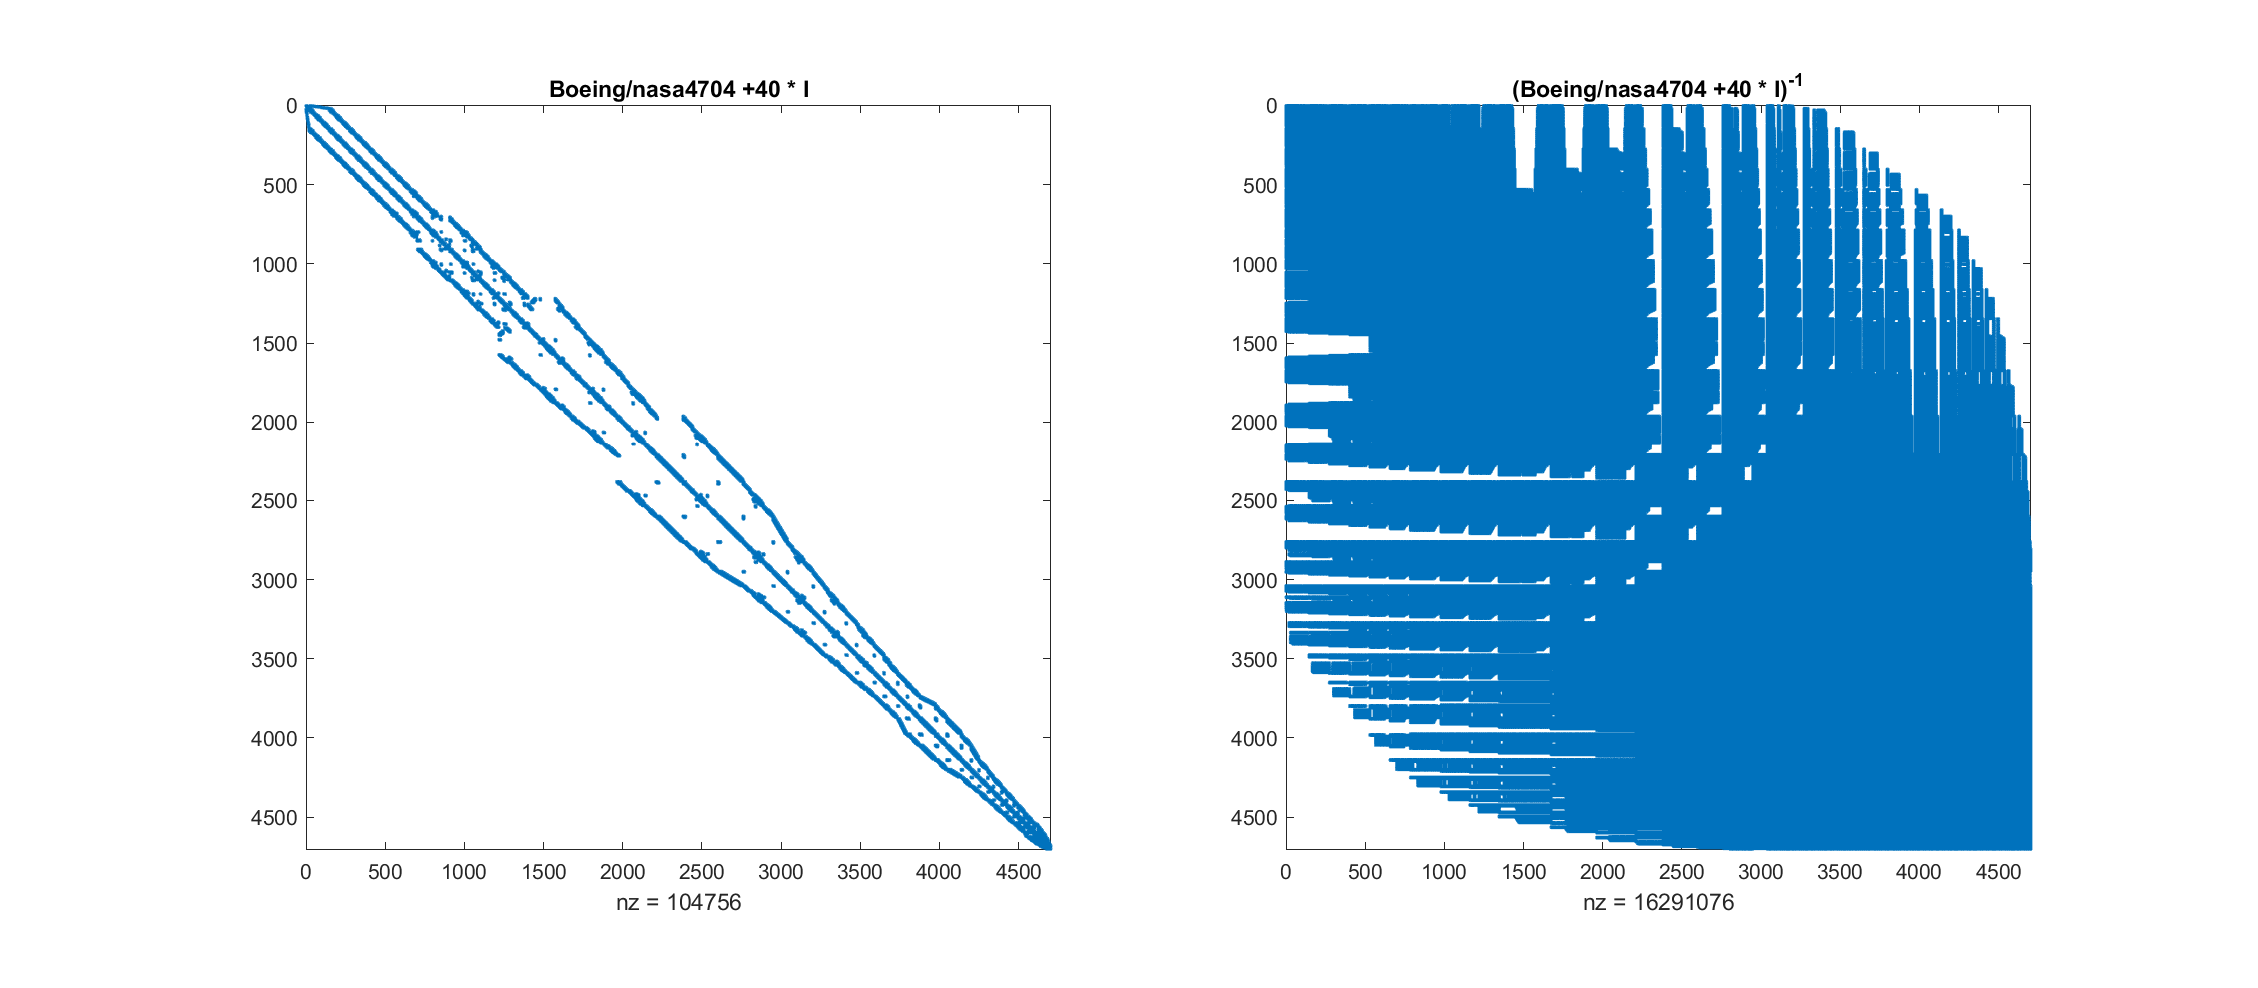
\includegraphics[width=\textwidth]{matrixandinversed.eps}
\caption{Wynik programu - struktura macierzy rozrzedzonej i jej odwrotności}
\label{fig:universe}
\end{figure}

\bibliographystyle{plain}
\bibliography{references}
\end{document}
